\chapter{Self-training for image segmentation}
\label{chap:strain}

\begin{overview}{Overview}
  In this chapter, \\
  
  \textbf{References:} this chapter is based on an article pending review \\
  
  Supplementary materials for this chapter can be found in Appendix Chapter \ref{app:strain}.
  \end{overview}

\section{Introduction}
\label{sec:strain:intro}

In this chapter, we investigate a method for training a binary image segmentation model in a context where the segmentation ground truth is sparse. More precisely, we focus on a setup where the training set is composed of an exhaustively-labeled subset $\mathcal{D}_l$ and a sparsely-labeled subset $\mathcal{D}_s$. In particular, the images in $\mathcal{D}_l$ come with exhaustively-labeled segmentation masks (\ie pixels of all objects of interest have been labeled as positive) whereas in $\mathcal{D}_s$, some (unknown) pixels belonging to objects of interest have not been labeled, hence the sparsity. Typically, image segmentation methods require that the training images come with exhaustive pixel-wise labels. In our setup, it would correspond to only using $\mathcal{D}_l$ and ignoring $\mathcal{D}_s$. We believe that it is possible to include the sparsely labeled images as well, and hopefully improve the performance of a segmentation model. One way of achieving this would be to somewhat ``complete'' the sparse segmentation masks and make them exhaustively labeled. Generating pseudo-labels is precisely what self-training approaches do and, in this work, we devise a self-training workflow to exploit both our sets.

Our self-training workflow consists of two separate phases. During the '\textit{warm-up}' phase, we train a U-Net \parencite{ronneberger2015unet} model in a classical supervised manner on $\mathcal{D}_l$ for a few epochs. Then, during the '\textit{self-training}' phase, we repeat the following process for an arbitrary number of epoch : pseudo labels are generated for the unlabeled pixels from images in $\mathcal{D}_s$ using the currently trained model and the pseudo-labeled images are included in the training set for the next epoch. To control the impact of model uncertainty on pseudo-labeled pixels, we furthermore study different weighting techniques to tune their contributions to the training loss. We study the use of both soft and hard pseudo-labels and propose an auto-threshold approach for generating the latter. We investigate the interest of our method and its hyperparameters in different scarcity conditions and compare it to different baselines. We also investigate a new dataset labeling strategy motivated by our setup in order to answer the question: at a fixed annotation budget, is it better to generate label exhaustive masks or a mix of exhaustive and sparse label masks ? To support our analysis, we use four datasets including the public \acrshort{monuseg} \parencite{kumar2019multi}, \acrshort{glas} \parencite{sirinukunwattana2017gland} and \acrshort{segpc} \parencite{gupta2021segpc} and one in-house sparsely-labeled dataset collected on Cytomine \parencite{maree2016collaborative}.  

When working with a dataset organized similarly to our setup ($\mathcal{D}_l$ and $\mathcal{D}_s$), we show that hard labels outperform soft labels (see Section \ref{ssec:strain:res:hardvssoft}) and that our self-training approach is beneficial as, even in significant scarcity conditions, it improves over using only exhaustively labeled data (only $\mathcal{D}_l$) in a fully supervised fashion (see Section \ref{ssec:strain:fixednl}). Surprisingly, we also observe that our self-training approach applied to a specific sparsified version of \acrshort{monuseg} is able to outperform the supervised baseline on the original fully labeled dataset (see Section \ref{ssec:strain:monuseganomaly}). However, we show that, at fixed annotation budget, it is better to focus the annotation effort on exhaustive labels rather than sparse labels (see Section \ref{ssec:strain:sparsevsexhaustive}).

Related works for this chapter can be found in Sections \ref{ssec:backml:dl:selftraining} and \ref{ssec:backdp:st}.


% Recent progresses in computing and artificial intelligence (AI) have created exciting opportunities the field of digital pathology. Nowadays, glass slides can be digitized into Whole-Slide Images (WSI) opening the way for AI-based analysis tools to relieve pathologists workload. Given the potentially dire consequences of misdiagnosis, these tools must be robust and reliable which can be challenging given the nature of the tasks and the different sources of variability affecting the WSI acquisition process. Machine learning techniques are considered some of the most promising tools to tackle these challenges but they often require a significant amount of training data to perform well. This is an issue in digital pathology which is considered to suffer from data scarcity \parencite{tizhoosh2018artificial, litjens2017survey}: high-quality annotated pathology data are expensive and difficult to obtain. 

% This is the case in particular for structured output tasks such as image segmentation as exhaustive pixel-wise image labeling is a tedious task. When it comes to reducing the labeling cost, several approaches have been explored over the years: reducing the cost per annotation (\eg crowd-sourcing through citizen-science \parencite{peplow2016citizen} or the intervention of junior pathologists and students \parencite{amgad2021nucls}), reducing the time per annotation (\eg active learning and human-in-the-loop \parencite{chai2020human}, dedicated annotation tools such as Cytomine \parencite{maree2016collaborative}, interactive annotation \parencite{berg2019}, or ai-assisted annotation \parencite{amgad2021nucls, graham2021conic, aubreville2021mitosis}) or reducing the quantity of annotations needed in the first place (\eg use of external data trough transfer learning \parencite{mormont2018comparison} or multi-task learning \parencite{mormont2020multi})

%In this work, we are interested in the third category. More precisely, in order to reduce the required amount of annotated data, we study a labeling scheme where only a small subset of the available training data has to be exhaustively labeled whereas the rest can only be sparsely labeled, \TODO{or even left unlabeled}.  We evaluate how this labeling scheme can be exploited by learning methods to train efficient segmentation models. This learning problem belongs to semi-supervised learning and we use a self-training approach to tackle it.


\section{Methods}
\label{sec:strain:methods}

In the following section, we present our method, a self-training image segmentation algorithm. The self-training aspects and training implementation details are discussed separately in Sections \ref{ssec:strain:self_training} and \ref{ssec:strain:training_protocol} respectively.

We will designate a segmentation dataset, or task, $\mathcal{D} = \left(X, Y\right) \subset \mathcal{X} \times \mathcal{Y}$ where $X \subset \mathcal{X}$ and $Y \subset \mathcal{Y}$ respectively represent the sets of input images and their corresponding binary segmentation masks. We will further consider a training dataset composed of two sets $\mathcal{D}_l = \left(X_l, Y_l\right) \subset \mathcal{X}_l \times \mathcal{Y}_l$, the exhaustively-labeled set, and $\mathcal{D}_s = \left(X_s, Y_s\right) \subset \mathcal{X}_s \times \mathcal{Y}_s$, the sparsely-labeled set. In $\mathcal{D}_l$, the masks $Y_l$ are entirely determined as the ground truth is known for all pixels (hence the exhaustiveness). In $\mathcal{D}_s$, ground truth is only partially known: given an image $\mathbf{x} \in X_s$, either a pixel $x_{ij}$ belongs to a structure of interest in which case the mask pixel $y_{ij} = 1$, or it is not labeled in which case $y_{ij} = 0$ and no assumption can be made a priori about the fact that the pixel belongs to a structure of interest or not. 

\subsection{Self-training}
\label{ssec:strain:self_training}
 
Our self-training algorithm is described in Algorithm \ref{algo:strain:selftraining}. It features a warm-up phase during which the model is classically trained on the set $\mathcal{D}_l$ (training implementation detail are given in Section \ref{ssec:strain:training_protocol}). The number of warm-up epochs $W > 0$ is fixed so that the model is able to converge on the labeled data. The warmed-up model is used as starting point for the self-training phase. Each self-training round $e$ starts by pseudo-labeling $\mathcal{D}_s$ with the model $\theta_{e-1}$. For an image $\mathbf{x} \in X_s$, the pseudo-label assigned to pixel $x_{ij}$ is given by:
\begin{equation}
y^{({pl})}_{ij} = \begin{cases}
1,\,\text{if}\, y_{ij} = 1 \\
g(\hat{y}_{ij}),\,\text{otherwise}
\end{cases}
\label{eqn:strain:pseudolabeling}
\end{equation}
where $\hat{y}_{ij}$ is the sigmoid output of model $\theta_{e-1}$ for pixel $(i, j)$ given $\mathbf{x}$ as input and $g$ is a function for generating the pseudo-label from $\hat{y}_{ij}$ (see Section \ref{sssec:strain:softandhardlabels}). In other words, we preserve the expert ground truth as pseudo-labels when available and use the model predictions for unlabeled pixels (this is the \texttt{Combine} step from Algorithm \ref{algo:strain:selftraining}). With this strategy, entirely unlabeled images can also be included in $\mathcal{D}_s$. Our algorithm uses a single model (\ie teacher = student) which is not reset between self-training rounds. This approach has been applied in other self-training contributions \parencite{laine2016temporal, bai2017semi, li2018based}. 

\begin{algorithm}[t]
  \SetAlgoLined
  \KwData{The exhaustively- and sparsely-labeled sets $\mathcal{D}_l$ and $\mathcal{D}_s$, a segmentation model $\theta_0$, $W$ and $E$ respectively the number of warm up epochs and the total number of epochs.}
  \KwResult{A self-trained segmentation model $\theta_E$.}
  \SetKwFunction{Train}{Train}
  \SetKwFunction{Predict}{Predict}
  \SetKwFunction{Combine}{Combine}
  // \textit{Warm up}  \\
  \For{$e \leftarrow 1$ \KwTo $W$}{
    $\theta_e$ = \Train{$\theta_{e-1}, \mathcal{D}_l$}\;
  }
  \For{$e \leftarrow W+1$ \KwTo $E$}{
    // \textit{Pseudo labeling} \\
    $\hat{Y}_s =$ \Predict{$\theta_{e-1}, X_s$}\;  
    $Y_{pl} =$ \Combine{$\hat{Y}_s, Y_s$}\; 
    $\mathcal{D}_{pl} = \left(X_s, Y_{pl}\right)$\; 
    // \textit{Self-training} \\
    $\theta_e$ = \Train{$\theta_{e-1}, \mathcal{D}_l \cup \mathcal{D}_{pl}$}\;
  }
  \KwRet{$\theta_E$}
  \caption{Our self-training approach. The \texttt{Train} operation trains the given model on the provided dataset according to the protocol explained in Section \ref{ssec:strain:training_protocol}. The \texttt{Predict} operation produces segmentation masks for a set of input images using the model. The \texttt{Combine} operation combines ground truth masks and pseudo labels from the given sets as explained in Section \ref{ssec:strain:self_training}.}
  \label{algo:strain:selftraining}
\end{algorithm}

\subsubsection{Soft and hard pseudo-labels}
\label{sssec:strain:softandhardlabels}

We study two different pseudo-labeling strategies, or two different $g$ functions (see Equation \ref{eqn:strain:pseudolabeling}). The first is simply taking $g$ to be the identity function $g(x) = x$ in which case the sigmoid output of the model is taken as pseudo-label. This strategy is commonly called  ``\textit{soft}'' labeling. During the next self-training round, this soft label will be compared to the network prediction which can be seen as a form of consistency constraint similar to those in \cite{laine2016temporal,tarvainen2017mean, sohn2020fixmatch}. The second strategy consists in thresholding the sigmoid output with $T_e \in [0, 1]$ in which case:
\begin{equation}
g(x) = \begin{cases}
1,\,\text{if}\, x > T_e\\
0,\,\text{otherwise}
\end{cases}
\end{equation}   
where $e$ is a self-training round. We call this strategy ``\textit{hard}'' labeling as pseudo-labels are either 1 or 0. In addition to ensuring some sort of consistency between the pseudo-labels and the predictions like the ``\textit{soft}'' approach does, this hard approach also encourages the model to produce confident predictions (close to 0 or 1). Because we want to avoid $T_e$ to be an additional hyperparameter to tune, we propose an auto-calibration strategy based on the Dice score: 
\begin{equation}
  Dice_T(\mathbf{y},\hat{\mathbf{y}}) = \dfrac{2 \times \sum_{i,j} \left[\mathbb{1}_{\hat{y}_{ij} \geq T} \times y_{ij}\right]}{\sum_{i,j} \mathbb{1}_{\hat{y}_{ij} \geq T} + \sum_{i,j} y_{ij}}
  \label{eqn:strain:dice}
\end{equation}
where $T$ is the threshold applied to the model output to generate a binary prediction. The auto-calibration procedure selects $T_e$ such the Dice score (see Equation \ref{eqn:strain:dice}) is maximized for the images from the labeled set $\mathcal{D}_{l}$:
\begin{equation}
T_e = \arg \underset{T}{\max} \sum_{(\mathbf{x}, \mathbf{y}) \in \mathcal{D}_l} \text{Dice}_T\left(\mathbf{y},h( \mathbf{x}; \theta_{e})\right).
\label{eqn:strain:thresholdopt}
\end{equation}
This auto-calibration has the advantage of not requiring additional training data compared to using an external annotated validation set for instance. However, it induces a risk of overfitting which might hurt generalization performance. In an extreme data scarcity situation, we argue that it is better to risk overfitting $\mathcal{D}_l$ than further reducing the size of the training set by extracting a validation set.

\subsection{Training}
\label{ssec:strain:training_protocol}

In this section, we will provide more information about the \texttt{Train} procedure from Algorithm \ref{algo:strain:selftraining} which trains a model $\theta$ with a dataset $\mathcal{D}$.
We use UNet \parencite{ronneberger2015unet} as a segmentation architecture. We set the initial number of features maps to 8 instead of 64 in the original article. The rest of the network is scaled accordingly. 

The number of rounds $W$ and $E$ and the number of training iteration per round are tuned independently per dataset. Every training iteration, we build a minibatch by sampling $B=8$ images uniformly at random with replacement from $\mathcal{D}$ and by extracting one randomly located 512x512 patch and its corresponding mask from each of these images. The batch size was selected based on hardware memory constraints. We apply random data augmentation following best practices for machine learning in general and for self-training in particular \parencite{xie2020self, sohn2020fixmatch}. We apply horizontal and vertical flips, color pertubation in the HED space \parencite{tellez2018whole} (bias and coefficient factors up to 2.5\%) \TODO{this augmentation was designed for H\&E images, 2 datasets out of 3 are not H\&E stained (thyroid, segpc)}, gaussian noise (standard deviation up to 10\%) and gaussian blur (standard deviation up to 5\%). 

As a training loss, we average the per-pixel binary cross-entropy $\ell$ over all pixels of the batch, as defined in:
\begin{align}
\ell(\hat{y}; y) = y \log \hat{y} + (1 - y) \log (1 - \hat{y}) \label{eqn:strain:perpixel_crossentropy} \\
\mathcal{L} = - \frac{1}{B} \sum_{b=1}^B \frac{1}{|\mathbf{y}_b|}\sum_{i}\sum_{j} w_{ij, b} \ell(\hat{y}_{ij, b}; y_{ij,b }) 
\label{eqn:strain:overallloss}
\end{align}

We multiply the per-pixel loss by a weight $w_{ij, b}$ for pixel $(i, j)$ of $b^{th}$ image of the batch in order to tune the contribution of this pixel to the loss (see Section \ref{sssec:strain:weights}). We use Adam \parencite{kingma2014adam} as an optimizer with initial learning rate $\gamma= 0.001$ and default hyperparameters ($\beta_1 = 0.9$, $\beta_2 = 0.999$, no weight decay).


\subsubsection{Weights}
\label{sssec:strain:weights}
In this section, we present the different strategies we evaluate for generating the per-pixel weight $w_{ij,b}$ in Equation \ref{eqn:strain:overallloss}. For the sake of simplicity, we will drop the batch identifier $b$ in the subsequent equations and denote this weight $w_{ij}$. We introduced this weight term to have a possibility to tune the contribution of pseudo-labeled pixels when computing the loss. It is important to note that this weight only applies to pseudo-labeled pixels and, therefore, the ground truth pixels will always be attributed a weight of $w_{ij} = 1$. It is also important to note that the weight is inserted as a constant in our loss and the weight function is not differentiated during back-propagation. 

We study five different weighting strategies each producing an intermediate weight $w^{\xi}_{ij}$ where $\xi$ is the strategy identifier. Because we want to avoid the amplitude of the loss to be impacted by the weighting strategy, we normalize it to obtain the final weight:
\begin{equation}
w_{ij} = \dfrac{w^{\xi}_{ij}}{\overline{w}^{\xi}}
\end{equation}
where $\overline{w}^{\xi}$ is the average weight over all pixels of a patch. Our five strategies are as follows:

\paragraph{Constant} This strategy consists in setting $w^{\text{cst}}_{ij} = C$ where $C \in \mathbb{R}^+$ is an hyperparameter. Because $w_{ij} = 1$ for ground truth pixels, this allows to manually balance the relative contributions of ground truth and pseudo-labeled pixels. The special case of $C = 1$ assigns the same weight to ground truth and pseudo-labels and therefore corresponds to removing $w_{ij,b}$ from Equation \ref{eqn:strain:overallloss}.

\paragraph{Balance} This strategy automatically assigns a value to the $C$ hyperparameter presented in the ``constant'' strategy. As a basis for this value, we use the ratio $g$ of ground truth pixels in $\mathcal{D}_l \cup \mathcal{D}_s$. The final weight is given by: 
\begin{equation}
w^{\text{bal}}_{ij} = \frac{g}{1 - g}.
\label{eqn:strain:balancegt}
\end{equation}
This choice is motivated by the belief that our algorithm will provide more reliable pseudo-labels in a low data scarcity regime ($g \nearrow $) in which case it makes sense to tune up the contributions of those pseudo-labels to the loss. In the opposite situation of extreme data scarcity ($g \searrow $), we expect the algorithm to produce less reliable pseudo-labels. 

\paragraph{Entropy} \label{par:strain:entropyweight} Unlike the previous ones, this strategy is not concerned with balancing the contributions but instead penalizes pseudo-labels for which the model was uncertain. It considers the prediction $\hat{y}_{ij}$ as a probability and tune the contribution down using the Shannon entropy. The use of entropy is motivated by its use in several self-training methods \parencite{grandvalet2004semi, lee2013pseudo}. First, an intermediate weight $\omega_{ij}$ is computed as: 
\begin{equation}
\omega_{ij} = 1 + \hat{y}_{ij} \log_2(\hat{y}_{ij}) + (1 - \hat{y}_{ij}) \log_2(1 - \hat{y}_{ij}).
\label{eqn:strain:entropyweight}
\end{equation}
Early experiments have shown that directly using $\omega_{ij}$ as a weight resulted in unstable training. Indeed, during early self-training rounds, the model typically produces $\hat{y}_{ij} \sim 0.5$ which results in $\omega_{ij} \sim 0$ for most pixels in a patch, leaving only foreground ground truth pixels to be evaluated in the loss. In order to avoid this behavior, we introduce a new hyper-parameter $w_{min} \in \left]0, 1\right]$ which allows rescaling linearly the weights $\omega_{ij}$ to $w^{ent}_{ij} \in [w_{min},1]$ as defined in:
\begin{equation}
w^{ent}_{ij} = \left(1 - w_{\text{min}}\right) \omega_{ij} + w_{\text{min}}.
\label{eqn:strain:wminrescale}
\end{equation}

\paragraph{Consistency} Self-training algorithms often enforce consistency between the teacher and student models predictions. Inspired from this, we exploit another form on consistency for this strategy. In structured output tasks like segmentation, there is a correlation between predictions that are spatially close, as, for most pixels, it is unlikely that the true label should differ between a pixel and its neighbors. Therefore, we use the pseudo-label consistency between a pixel and its neighbors as a proxy to evaluate reliability of this pseudo-label. The weight is given by
\begin{equation}
w^{\text{cty}}_{ij} = 1 - \dfrac{\sum_{k=-\eta}^{\eta} \sum_{l=-\eta}^{\eta} c(\hat{y}_{ij},  \hat{y}_{(i+k)(j+l)})}{\eta^2 - 1}
\end{equation}
where $c(y_1,y_2)$ is a consistency function for a pair of pixel and $\eta$ is the size of the neighborhood. Both are hyperparameters of the method. Regarding $\eta$, we consider a square neighborhood around the central pixel. Therefore, when $\eta = 1$ and $2$, 8 and 24 pixels are respectively compared to the central pixel. When consistency is computed on the image border, we ignore pixels outside of the image.

% \begin{figure}
%     \centering
%     \includegraphics[scale=0.325]{images/neighbourhood.png}
%     \caption{Neighbourhood parameter $\eta$.}
%     \label{fig:strain:neighbourhood}
% \end{figure}

\paragraph{Merged} This strategy assigns a high weight to pixels for which the model is both certain and consistent (spatially). It achieves this by multiplying together the consistency weight $w^{\text{cty}}_{ij}$ and the entropy raw weight $\omega_{ij}$. Because $\omega_{ij}$ suffers from the issue described earlier, we apply the same re-scaling operation after multiplication:
\begin{equation}
w^{\text{mgd}}_{ij} = (1 - w_{min}) \left(w^{\text{cty}}_{ij} \times \omega_{ij}\right) + w_{min}.
\end{equation}


\section{Data}
\label{sec:strain:data}
In this section, we describe the datasets we use to evaluate our method. It includes three public datasets (see Section \ref{ssec:strain:datapublicdatasets}) and an in-house sparsely-annotated dataset which has initially motivated this work (see Section \ref{ssec:strain:thyroidfnab}). 

\subsection{\acrshort{monuseg}, \acrshort{glas} and \acrshort{segpc}}
\label{ssec:strain:datapublicdatasets}
We use 3 exhaustively-annotated public segmentation datasets for this purpose.

\acrshort{monuseg} \parencite{kumar2019multi} contains 44 images coming from different organs, patients and hospitals with a total of 28846 annotated epithelial and stromal nuclei. The dataset is split into some training (30 images, 17362 cells) and test (14 images, 11484 cells) sets. Each image contains a significant number of cell annotations (few hundreds to a thousand) of which the dimensions are quite uniform. As for the images, they show great variations of appearance given the variety of sources. See Figures \ref{sfig:strain:monuseg_sample1} and 
\ref{sfig:strain:monuseg_sample2} for samples.

\acrshort{glas} \parencite{sirinukunwattana2017gland} contains 85 training and 80 test images with binary segmentation masks of intestinal glands. The image contains both benign tissue as well as colonic carcinomas. The gland annotations vary greatly in shape and size. These variations can be caused by the presence of a carcinoma or simply the axis of cut of the tissue during the slide preparation. See Figures \ref{sfig:strain:glas_sample1} and 
\ref{sfig:strain:glas_sample2} for samples.  

\acrshort{segpc} \parencite{gupta2021segpc} contains 2633 annotated plasma cells over 498 annotated images. The original segmentation problem features 3 classes: background, cytoplasm and nucleus. In this work, we merge the two latter classes as we are only interested in binary segmentation. Only the training (298 images) and the validation sets are publicly available (200 images). One of the challenges of this dataset is the presence of non-plasma cells which should be ignored by the algorithm although they are very similar to plasma cells. Moreover, artefacts are present on the images (\eg cracked scanner glass in foreground, scale reference or magnification written on the image). See Figures \ref{sfig:strain:segpc_sample1} and \ref{sfig:strain:segpc_sample2} for samples.

\begin{figure}
  \centering
  \begin{subfigure}{0.48\textwidth}
    \centering
    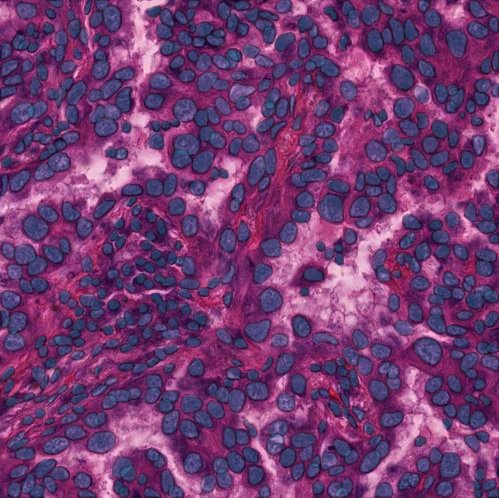
\includegraphics[width=\textwidth]{strain/monuseg_sample1.png}
    \caption{\acrshort{monuseg}}
    \label{sfig:strain:monuseg_sample1}
  \end{subfigure}
  \begin{subfigure}{0.48\textwidth}
    \centering
    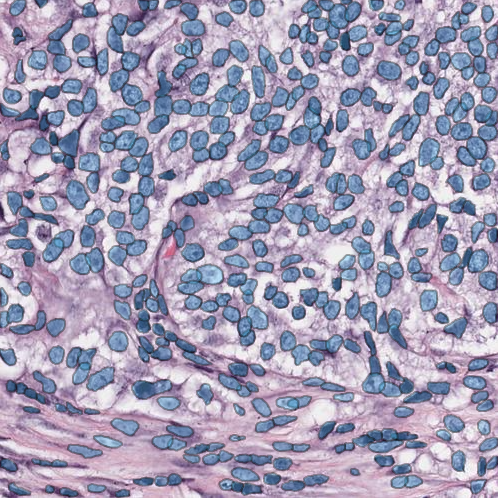
\includegraphics[width=\textwidth]{strain/monuseg_sample2.png}
    \caption{\acrshort{monuseg}}
    \label{sfig:strain:monuseg_sample2}
  \end{subfigure} \\

  \begin{subfigure}{0.48\textwidth}
    \centering
    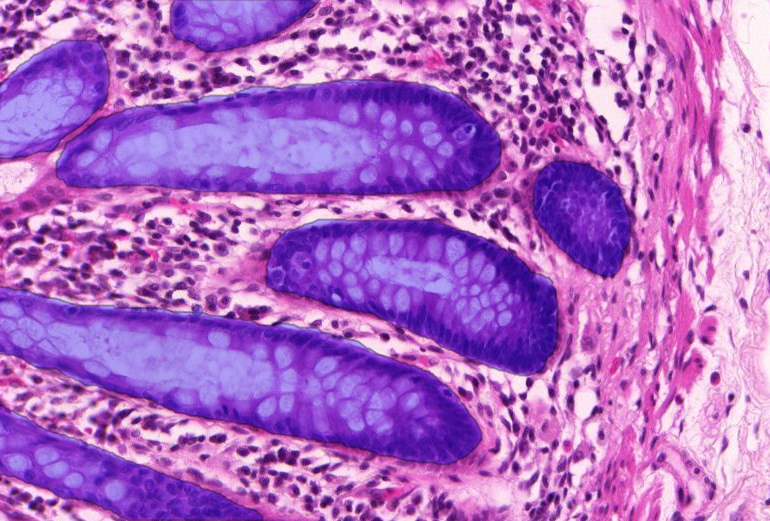
\includegraphics[width=\textwidth]{strain/glas_sample1.png}
    \caption{\acrshort{glas}}
    \label{sfig:strain:glas_sample1}
  \end{subfigure}
  \begin{subfigure}{0.48\textwidth}
    \centering
    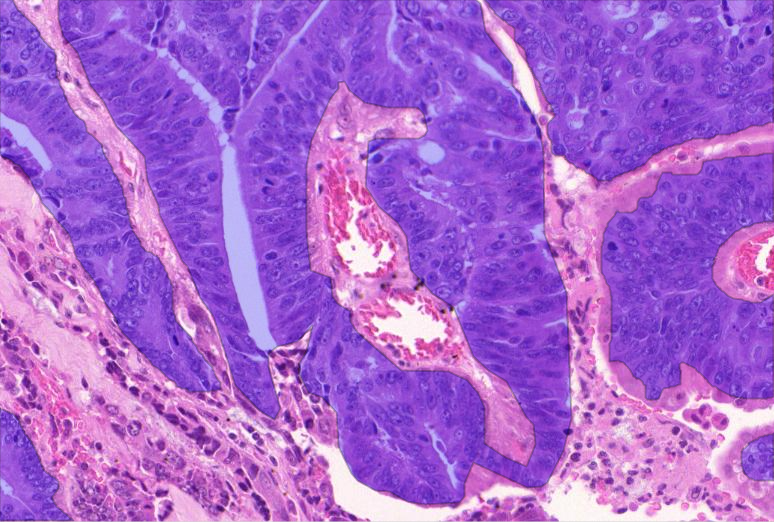
\includegraphics[width=\textwidth]{strain/glas_sample2.png}
    \caption{\acrshort{glas}}
    \label{sfig:strain:glas_sample2}
  \end{subfigure} \\

  \begin{subfigure}{0.48\textwidth}
    \centering
    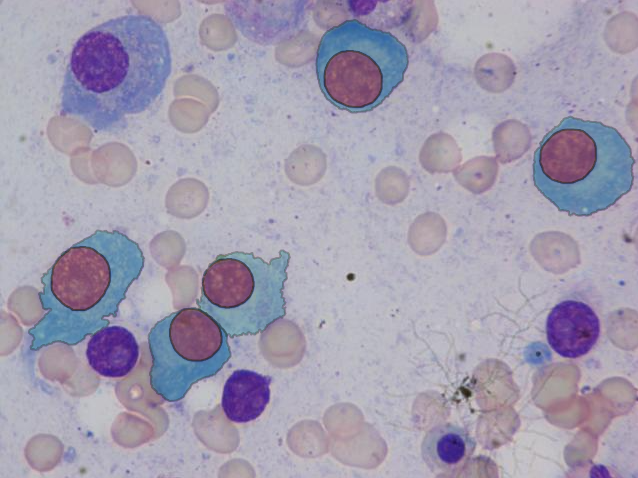
\includegraphics[width=\textwidth]{strain/segpc_sample1.png}
    \caption{\acrshort{segpc}}
    \label{sfig:strain:segpc_sample1}
  \end{subfigure}
  \begin{subfigure}{0.48\textwidth}
    \centering
    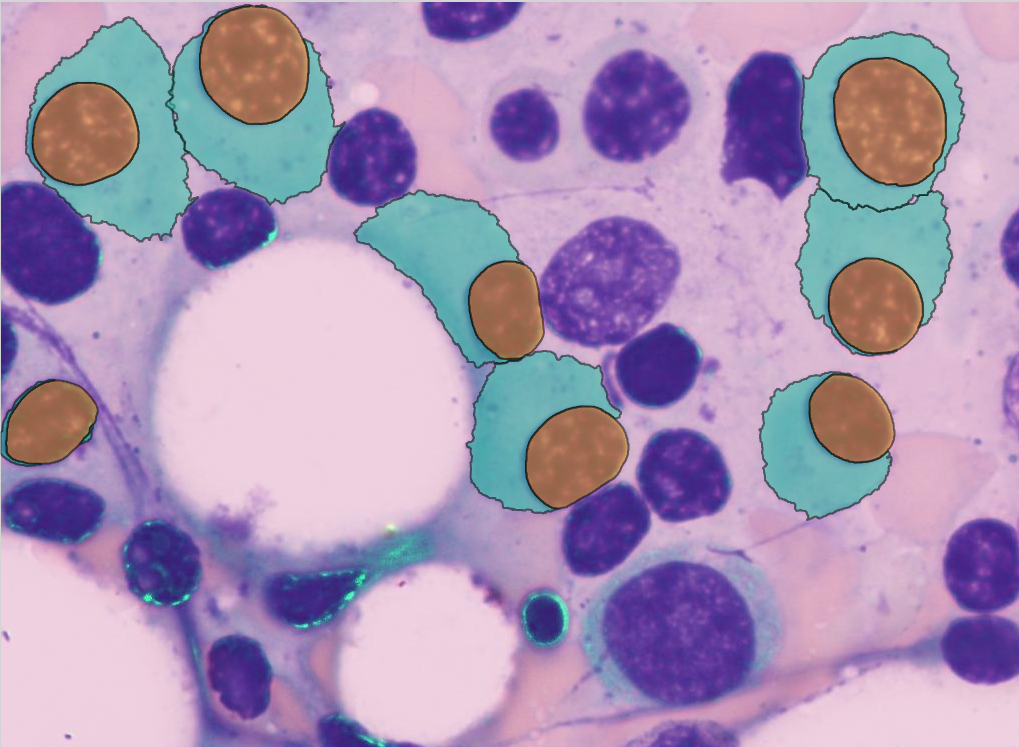
\includegraphics[width=\textwidth]{strain/segpc_sample2.png}
    \caption{\acrshort{segpc}}
    \label{sfig:strain:segpc_sample2}
  \end{subfigure} 
  
  \caption{Samples from \acrshort{monuseg}, \acrshort{glas} and \acrshort{segpc} used in this work.}
  \label{fig:strain:datasets_samples}
\end{figure}


\subsection{Thyroid \acrshort{fnab}}
\label{ssec:strain:thyroidfnab}

We use an in-house sparsely-annotated dataset collected on the Cytomine platform. This dataset contains a set of 81 WSIs with fine-needle aspiration biopsies (\acrshort{fnab}) from thyroid nodules stained with Diff-Quik. These images were digitized using \TODO{several scanners (Aperio, Hammamatsu)???} at a 0.226 $\mu m$/pixel resolution and uploaded to Cytomine. 

Expert pathologists from the ULB Erasme hospital (Brussels, Belgium) highlighted structures of interest in these WSIs using polygon annotations. These structures can be broadly grouped into two categories: nuclear features (individual nuclei or cells) and architectural patterns (groups of cells). Both categories contain malignant and healthy entities. \TODO{(not sure if necessary to include)The complete ontology can be found in Table??}. The pathologists were not given any precise directions during the labeling process. Therefore, they navigated the images and, as they went, annotated examples of the ontology terms. They did not exhaustively annotate any region of interest. The resulting annotations can therefore be considered sparse as can be seen in Figure \TODO{???}. 

% \begin{figure*}
%   \centering
%   \subfloat[Nuclear feature 1]{\includegraphics[height=87.5pt]{images/nuclfeatures_sparse.png}}
%   \hspace{3pt}
%   \subfloat[Nuclear feature 2]{\includegraphics[height=87.5pt]{images/nuclfeatures_sparse2.png}}
%   \hspace{3pt}
%   \subfloat[Nuclear feature 3]{\includegraphics[height=87.5pt]{images/nuclfeatures_sparse3.png}}
%   \hspace{3pt}
%   \subfloat[Architectural patterns]{\includegraphics[height=87.5pt]{images/archpattern_sparse.png}}
%   \caption{Example annotations of nuclear features and architectural patterns captured on Cytomine. Notice the sparseness of the annotations.}
%   \label{fig:strain:thyroid_example_annotations}
% \end{figure*}

The dataset we use in this work was generated from these annotations. In particular, we have extracted crops centered around each annotation of interest with a minimum image size of 512 $\times$ 512 pixels at maximum resolution. If the annotation was larger than that, the crop was built to contain exactly the annotation. We are interested in binary segmentation therefore, for each crop image, we have extracted a binary mask where each pixel $y_{ij}$ is labeled $1$ (foreground) if it is contained in an annotated object (whether or not this object is the cropped annotation) and the rest of them are assigned label $0$ (background). The resulting dataset contains 4742 crops with 3003 nuclear features and 1739 architectural patterns. 

In order to evaluate the method, a computer science student exhaustively annotated 20 validation and 25 test regions of interest of 2000x2000 pixels on Cytomine. The anotations are binary and correspond to the type of problem resulting from assembling all terms into one foreground class. 


\section{Experimental setup}
\label{sec:strain:experiments}

In this section, we describe the experiments we have run and their results. These experiments aim at evaluating how our self-training approach performs against different baselines on the datasets described in Section \ref{sec:strain:data}. Moreover, we study the impact of different hyperparameters of our methods on the performance.

\subsection{Transforming the datasets}

In order to fit the sparsely-annotated settings described in Section \ref{sec:strain:methods}, we generate new datasets from \acrshort{segpc}, Glas and \acrshort{monuseg}. Because we want to study the effects of varying levels of sparsity, we randomly pick a certain amount of images $n_l$ for the set $\mathcal{D}_l$ and the rest are added to the set $\mathcal{D}_s$. To make the masks in $\mathcal{D}_s$ sparse, we randomly remove a certain percentage $\rho$ the annotated instances. For \acrshort{monuseg}, we remove $\rho$ \% of the instances in each image. For \acrshort{segpc} and Glas, because the number of instances per image is small, we remove $\rho$ \% of the instances from the complete list of instances. As a result, some training images can be missing ground truth. We study different values of $\rho$ and $n_l$ to evaluate the behavior of the method with different levels of sparsity.

Because the thyroid dataset is sparse from the start, we cannot adopt the same strategy and therefore keep it as-is. In order to fit the sparsely-annotated settings, we hypothesize that crops of nuclear features are more likely to be sparse than the crops of architectural patterns given the annotation process. Therefore, we use the former set as $\mathcal{D}_s$ and the latter as $\mathcal{D}_l$.

\subsection{Baselines}

We compare our self-training approach to three baselines. The first consists in using the full dataset, without removing any ground truth (\ie $|\mathcal{D}_s| = 0$). Given that our experiments are performed on versions of the datasets where annotated instances were removed, this first baseline should be an upper-bound on the performance of self-training. The second consists in using the sparsely-annotated set $\mathcal{D}_s$ as if it was exhaustively annotated ($\mathcal{D}_{train} = \mathcal{D}_l \cup \mathcal{D}_s$). This strategy makes sense especially for moderately sparse datasets. Indeed, convolutional layers (which compose UNet) are able to cope with a bit of label noise given that gradients are averaged over feature maps to update the parameters. Therefore, a bit of noise in certain parts of the images can be compensated by the feedback of ground truth labels in other locations. The last baseline consists in not using the sparsely-annotated images during the training process (\ie $\mathcal{D}_{train} = \mathcal{D}_l$). Our self-training approach is of interest if it outperforms the two latter baselines, moreover, the closer to the first baseline the better.

\subsection{Hyperparameters study}

Our self-training approach and our weighting strategies in particular come with a set of hyperparameters that we study in different scarcity conditions on the three datasets. In general, we will list the studied values alongside the associated results in the relevant sections (see Section \ref{sec:strain:results}). In this section, we comment and motivate the choices of hyperparameters values in general. 

Regarding the ``\textit{constant}'' strategy, we study $C \in \left\{0.01, 0.05, 0.1, 0.25, 0.5, 1, 1.5, 2\right\}$ to cover a wide range of possible $C$ values. The specific value $C = 1$ corresponds to to the absence of weights in the loss. We only consider other values of $C < 1$ because we believe that, especially in hard scarcity conditions, pseudo-labels can only impact negatively the training process so it makes sense to tune down their contributions to the loss. 

As a consistency function $c(y_1, y_2)$, we study both the absolute error $|y_1-y_2|$ and the squared error $(y_1-y_2)^2$. For the size of the neighborhood, we study $\eta \in \left\{1, 2\right\}$ which corresponds to the smallest possible neighborhoods. This ensures that the close pixels labels consistency assumption holds except at the very close vicinity of instance boundaries and to keep the computational cost of the method under control.

Regarding the minimum weight for the ``\textit{entropy}'' and ``\textit{merged}'' strategies, we evaluate $w_{\text{min}} \in \left\{0.01, 0.05, 0.1, 0.25, 0.5, 0.75\right\}$. These values were picked following the same motivations as hyperparameter $C$. The case $w_{min} = 1$ is not considered as it falls back to the case $C = 1$ with the ``\textit{constant}'' strategy discussed earlier.

\subsection{Evaluation}
\label{ssec:strain:evaluation}

We have built an evaluation protocol in order to ensure a fair comparison between the different strategies and the baselines. Ultimately, all approaches must produce a model $\theta$ and a threshold $T \in [0, 1]$ which we use to evaluate the model on the test sets of the datasets. We compare the test masks against the thresholded output of model $\theta$ for images of the test sets using the Dice score (see Equation \ref{eqn:strain:dice}). 

For all experiments except the $|\mathcal{D}_s| = 0$ baseline, we select as $\theta$ the model produced by the last training round and tune the threshold on $\mathcal{D}_l$ similarly as for the hard label strategy (see Equation \ref{eqn:strain:thresholdopt}). As mentioned earlier, tuning the threshold on the training data entails a risk of overfitting. However, in a context of extreme data scarcity, it is not always possible to obtain a sufficiently large validation set to tune this threshold. Therefore, we believe it is a realistic choice to use $\mathcal{D}_l$ as the tuning set.  

For the $|\mathcal{D}_s| = 0$ baseline, we have access to the fully annotated datasets and therefore can rely on more classical evaluation and tuning protocols. In this case, we extract approximately 10\% of the training images and masks to build a validation set. We evaluate the model every training round on this validation set using the Dice score. As a final model $\theta$ and threshold $T$, we select the model which yielded the best Dice score and its corresponding threshold. 

Every experiment and hyper-parameter combination we evaluate is run with ten different random seeds to evaluate the variability. The seed affects the dataset sparsification, model initialization, mini-batch sampling and data augmentation. In the case of the $|\mathcal{D}_s| = 0$ baseline, the seed affects the selection of the validation set. 

In the following sections, we report test Dice average and standard deviation over these random seeds.  

\paragraph{Manual threshold tuning} As previously explained, we tune the threshold on $\mathcal{D}_l$ for most experiments which implies a risk of overfitting. Therefore, we wanted to try another strategy. In practice, one could imaging a setup where a human would run the algorithm and generate $\theta$ then set $T$ by tuning it manually on a few test images. This protocol raises questions related to bias (human-related) and small sample size but depending on the final application (\eg \acrshort{ai}-assisted annotation), they might not really be an issue. This protocol would also alleviate the issue of training set overfitting. 

Therefore, we have re-evaluated the models generated during our experiments using a similar protocol similar to leave-one-out cross-validation. Given a run of our algorithm, we have extracted the final model $\theta$ and the associated random seed $r$. The seed was used to randomly extract $K$ images from the related test set $\mathcal{D}_t$ which were used to tune the threshold $T$. For the sake of simplicity, instead of using a human, we have applied the same threshold optimization procedure based on the Dice score as presented in Section \ref{sssec:strain:softandhardlabels} for hard labels. The threshold was then used to evaluate the model on the remaining $|\mathcal{D}_t| - K$ images. We have repeated this procedure for all seeds and then average the results. This process is similar to a non-exhaustive $K$-fold cross validation. 

\paragraph{Test set threshold optimization} Another way to evaluate the threshold without taking the risk of overfitting the training set would be to actually take $T$ such that the Dice score is maximized on the test set. This approach is not realistic in an extreme data scarcity situation as it would require a fully annotated test set (in our experiments, the test sets are almost always larger than the training set). However, we have still decided to evaluate the performance of the models using this approach to evaluate how much our first threshold generation method (\ie on $\mathcal{D}_l$) suffers from overfitting.   

\section{Experiments and results}
\label{sec:strain:results}

\subsection{Hard labeling \vs soft labeling}
\label{ssec:strain:res:hardvssoft}

In this section, we explore how the two choices of pseudo-label generation presented in Section \ref{sssec:strain:softandhardlabels} impact the performance of self-training. In order to answer this question, we have run our self-training approach a significant number of times with different hyperparameter settings either with hard or soft pseudo-labels. We have performed 10 runs per hyperparameter combination and with total of 45 combinations for \acrshort{segpc}, 42 for \acrshort{monuseg} and 22 for \acrshort{glas} (see Supplementary Section \ref{app:strain:hyperparameters_selftrain} for a detailed list of hyperparameters combinations). Regarding sparsity, we have decided to study a relatively scarce regime with $\rho = 90\%$ for all datasets and $n_l$ set to $2$ for \acrshort{monuseg}, $30$ for \acrshort{segpc} and $8$ for \acrshort{glas} (\ie between $90\%$ and $95\%$ of sparsely labeled images with $90\%$ of missing annotations).    

We observe that hard labels consistently yield superior performance on all datasets. 

\TODO{what if optimizing on test set?? way better perf for soft relatively to hard}
\begin{figure}
  \centering
  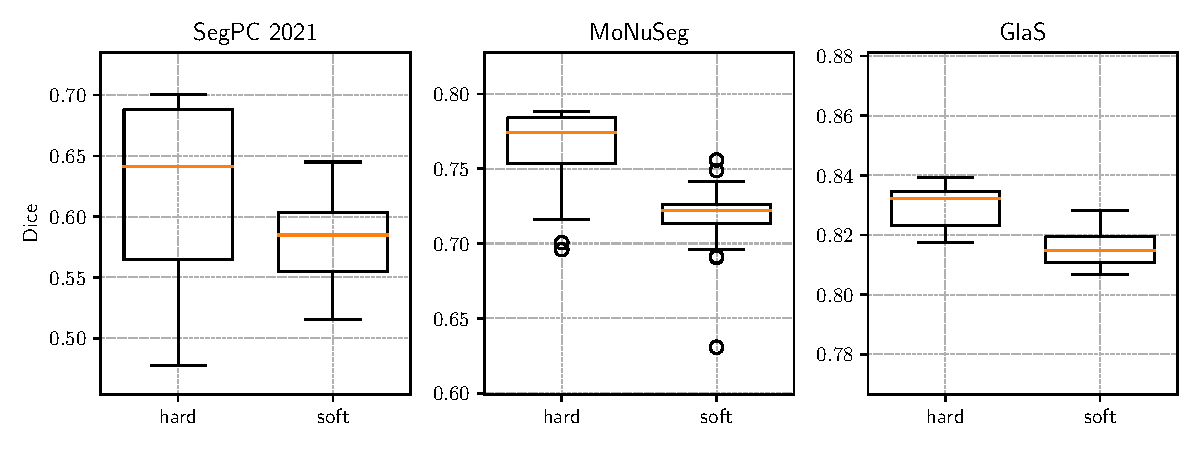
\includegraphics[width=\textwidth]{strain/plot_hard_vs_soft_test_hard_dice.pdf}
  \caption{Comparing performance between using self-training with hard \vs soft labels. The reported Dice score is optimized on $\mathcal{D}_l$.}
  \label{fig:strain:hard_vs_soft}
\end{figure}

\subsection{Self-training performance at fixed $n_l$}
\label{ssec:strain:fixednl}

In order to study how our self-training approach performs under different data scarcity regime, we have performed the following experiment. We have generated several versions of our datasets by varying $\rho$ with $n_l$ fixed and have run the baselines and different hyperparameters combinations on the generated datasets. Given the results of Section \ref{ssec:strain:res:hardvssoft}, we have used hard labels exclusively. The reported Dice scores are optimized on the test set. For all datasets, the upper baseline, $|\mathcal{D}_s| = 0$, outperforms the two others. 

\begin{figure}
  \centering
  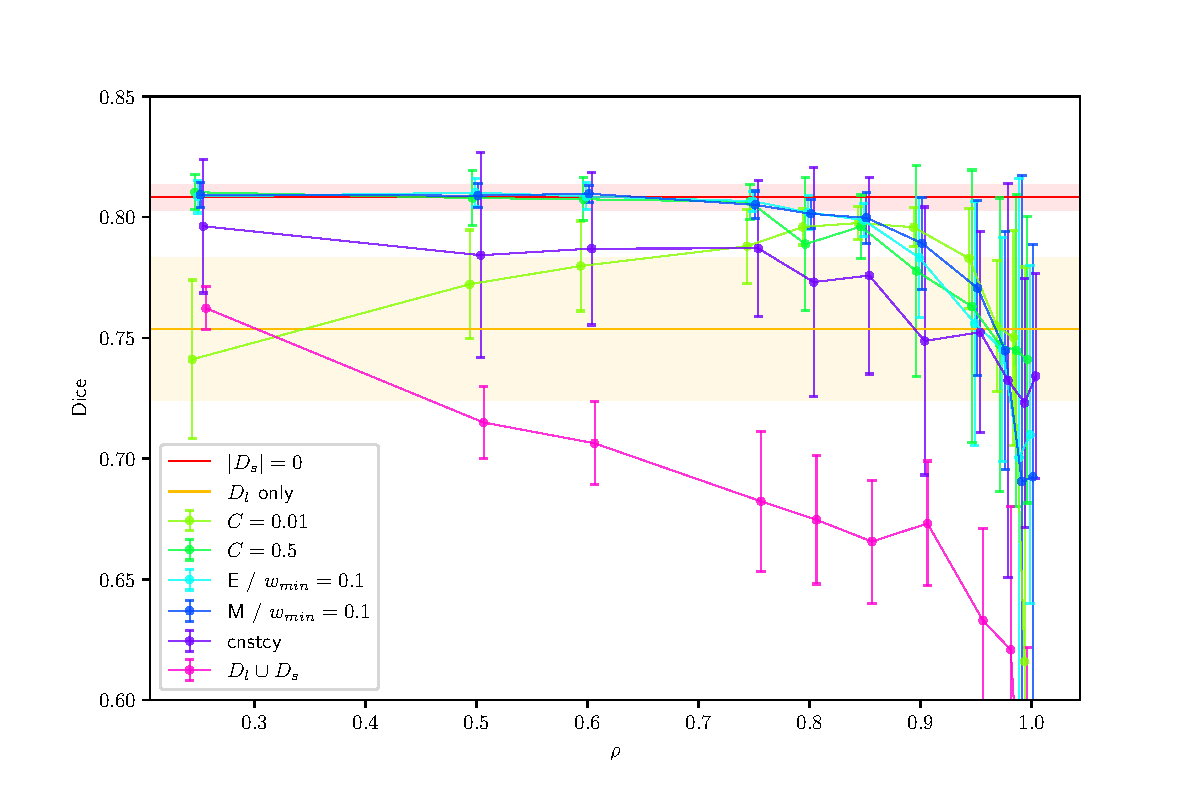
\includegraphics[width=0.9\textwidth]{strain/monuseg_test_pxl_self_hard_dice_rho_limTrue_errTrue.pdf}
  \caption{Performance of our baselines and self-training approaches with different hyperparameters combinations with a varying $\rho$ and a fixed labeled set size $n_l$ on \textbf{\acrshort{monuseg}}. ``$E / w_{min} = 0.1$'', ``$M / w_{min} = 0.1$'' and ``\textit{cnstcy}'' respectively stand for the entropy, merged (both with the specified $w_{min}$) and consistency weighting strategies. ``$C = 0.1$'', for instance, stands for the constant weighting strategy with the specified value as constant. The baselines are $|\mathcal{D}_s| = 0$, $\mathcal{D}_l$ only, $\mathcal{D}_l \cup \mathcal{D}_s$. The scores are obtained by optimizing the threshold $T$ on the test set.}
  \label{fig:strain:rho_exp_monuseg}
\end{figure}

\paragraph{\acrshort{monuseg}} First, on \acrshort{monuseg} (see Figure \ref{fig:strain:rho_exp_monuseg}), it is interesting to note that using sparsely labeled images as if they were exhaustively labeled (\ie baseline $\mathcal{D}_l \cup \mathcal{D}_s$) is generally not a good idea as it is outperformed by all other approaches in most cases. However, we observe that the performance of this baseline increase as one adds more sparse labels in $\mathcal{D}_s$ (\ie $\rho$ decreases), even making it more efficient than ``$\mathcal{D}_l$ only'' at $\rho = 25\%$. 

Then, we can divide the analysis by differentiating three scarcity regimes: extreme ($\rho \in [95\%, 100\%]$), significant ($\rho \in [80\%, 90\%]$) and medium ($\rho \in [25\%, 75\%]$). Overall, most self-training approaches benefit from additional sparse annotations as their score increase when $\rho$ decreases. This statement is true for all weighting strategies but the ``constant'' with $C = 0.1$ which plateau near $\rho = 85\%$, before decreasing as $\rho$ decreases. 

In the extreme regime, all self-training approaches exhibit high variance and are outperformed by the ``$\mathcal{D}_l$ only'' baseline, or yield comparable performance. In this situation, it appears to be better to work in a fully supervised fashion using only images from $\mathcal{D}_l$ rather then using our self-training approach. Indeed, it seems that the noise brought by the extreme annotation sparsity (or complete lack of annotation when $\rho = 100\%$) degrades the model significantly which cannot even make efficient use of the exhaustively labeled images anymore. For $\rho = 95\%$, two self-training approaches (``constant'' with $C = 0.1$ and ``entropy'') are on average better then the baseline but variance is still high making it difficult to really conclude that they are more efficient. 

The situation is reversed in the significant regime where most self-training approaches (except the ``consistency'' weighting strategy) outperform the ``$\mathcal{D}_l$ only'' baseline and variance decreases significantly as well. As for the $|\mathcal{D}_s| = 0$ baseline, it remains more efficient than self-training. For $\rho = 0.9$, the most efficient weighting strategy on average is ``constant'' with $C = 0.1$ which also exhibits the smallest variance of all the self-training approaches. We believe that such a low constant is particularily helpful to combat the noise brought by the high sparsity as pseudo-labeled pixels contribute way less during training. For $\rho = 85\%$ and $90\%$, the ``constant'' with $C = 0.1$ strategy plateaus whereas others catch up in terms of performance and variance decrease with the ``entropy'' and ``merged'' approaches taking up the lead.

In the medium regime, three self-training approaches reach, and even slightly surpass, the upper baseline: ``constant'' with $C = 0.5$, ``entropy'' and ``merged''. This result is interesting because it means that our self-training approach is able to reach the performance of a fully supervised approach but using only $\sim 30\%$ of the orignal annotations (\ie $\rho = 75\%$, approximately 5k annotations instead of 17k) which is a very significant annotation budget saving. The approach ``constant'' with $C=0.1$ scores decreases with $\rho$ indicating that such a low constant prevents the model to learn efficiently from the additional annotations (compared to the significant regime). This strategy even finished below the $\mathcal{D}_l \cup \mathcal{D}_s$ baseline at $\rho = 25\%$. 

Overall, result on MonuSeg are quite satisfactory. Although our approach is struggling in an extreme scarcity regime, it quickly catches up with the upper baseline as one adds more annotations to $\mathcal{D}_s$. In this case, the choice of weighting strategy matters and depends on the sparsity of the dataset.

\begin{figure}
  \centering
  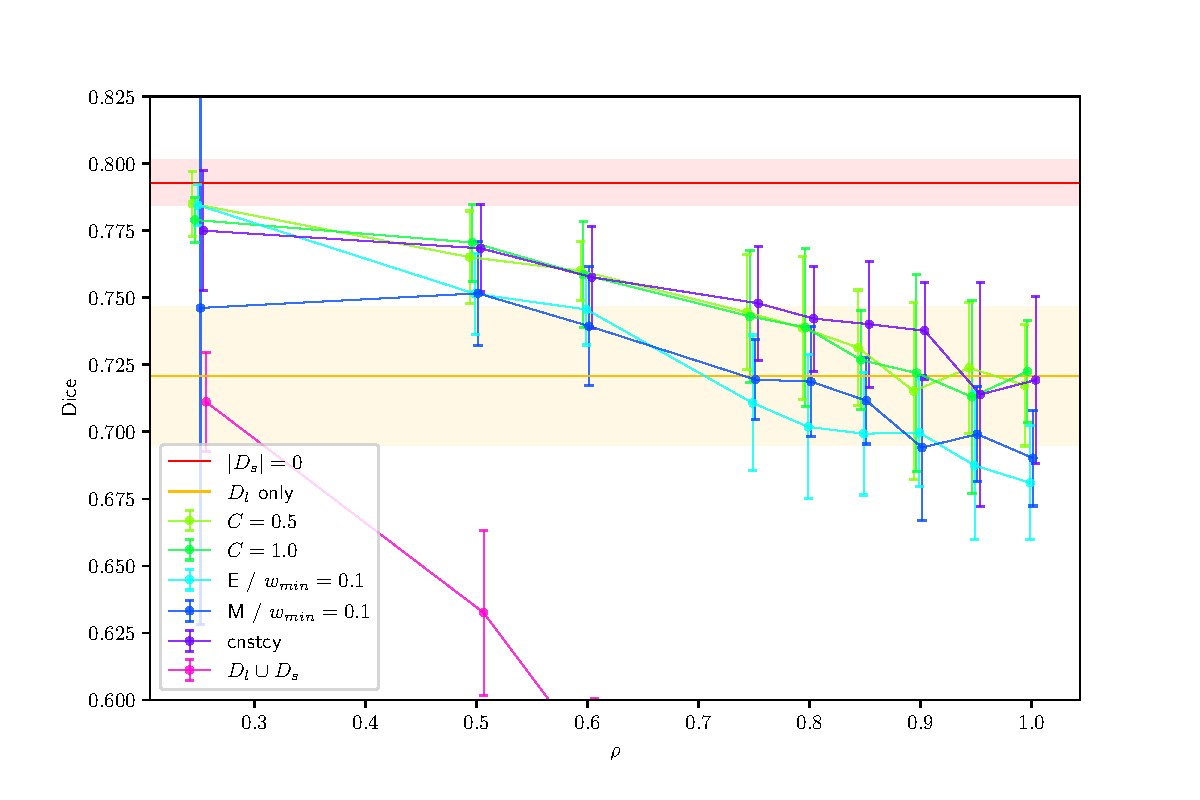
\includegraphics[width=0.9\textwidth]{strain/segpc_test_pxl_self_hard_dice_rho_limTrue_errTrue.pdf}
  \caption{Performance of our baselines and self-training approaches with different hyperparameters combinations with a varying $\rho$ and a fixed labeled set size $n_l$ on \textbf{\acrshort{segpc}}. See Figure \ref{fig:strain:rho_exp_monuseg} for explanation. The baseline $\mathcal{D}_l \cup \mathcal{D}_s$ performs significantly worse than all approaches and is therefore out of the range of interest. \TODO{show full range in appendix?}}
  \label{fig:strain:rho_exp_segpc}
\end{figure}

\paragraph{\acrshort{segpc}} Regarding the trend, our self-training approach behaves similary on \acrshort{segpc} (see Figure \ref{fig:strain:rho_exp_segpc}) compared to \acrshort{monuseg}: all self-training without exceptions seem to benefit from additional annotations in $\mathcal{D}_s$. Moreover, the $\mathcal{D}_l \cup \mathcal{D}_s$ baseline is particularily inefficient and finishes just below the ``$\mathcal{D}_l$ only'' baseline at $\rho = 25\%$. However, in the extreme regime, the gap between self-training and the ``$\mathcal{D}_l$ only'' baseline is less than compared to \acrshort{monuseg}. The rate at which our approach improves over the ``$\mathcal{D}_l$ only'' is also slower as it takes a larger $\rho$ (around $75\%$) for the performance of self-training to become significantly better than this baseline. The best-performing weighting strategies also differ. The best strategies overall are ``constant'' (with $C = 0.5$ or $1$) and ``consistency''. The ``merged'' and ``entropy'' are worse than the others, although the latter catches up at $\rho = 25\%$. Unfortunately, on this dataset, the self-training approaches are not able to reach the upper baseline. 

\begin{figure}
  \centering
  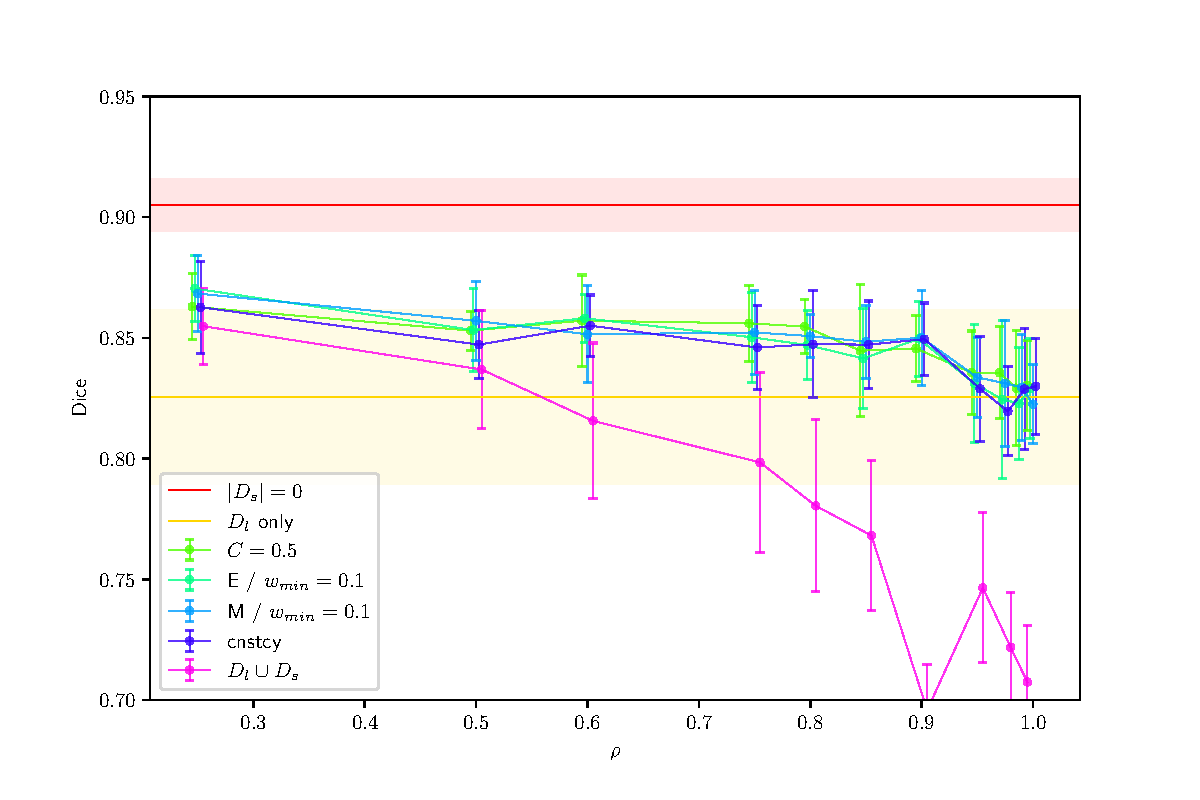
\includegraphics[width=0.9\textwidth]{strain/glas_test_pxl_self_hard_dice_rho_limTrue_errTrue.pdf}
  \caption{Performance of our baselines and self-training approaches with different hyperparameters combinations with a varying $\rho$ and a fixed labeled set size $n_l$ on \textbf{\acrshort{glas}}. See Figure \ref{fig:strain:rho_exp_monuseg} for explanation.}
  \label{fig:strain:rho_exp_glas}
\end{figure}

\paragraph{\acrshort{glas}} Before diving in the analysis for \acrshort{glas} (see Figure \ref{fig:strain:rho_exp_glas}), it is important to remember that there are much more variability in the shape and size of the annotations in this dataset. Therefore, removing an annotation versus another can lead to a very different outcome in terms of loss of information and actual sparsity increase. This might explain why the overall performance trend differs compared to the two other datasets. Indeed, in this case, the benefit from adding new annotations in $\mathcal{D}_s$ is less obvious as the performance curve for the self-training approach is flatter. Although, the self-training approaches are better than this baseline on average for most data points, the variance is such that the performance are mostly confounded until until $\rho = 25\%$.

\subsection{The \acrshort{monuseg} anomaly, when sparse is better than exhaustive}
\label{ssec:strain:monuseganomaly}

\TODO{already observed in the previous experiment with even less data????}

Among the experiments we have run, there is a specific sparsity condition that gave surprising results. This setup is $n_l = 15$ and $\rho = 90\%$ on \acrshort{monuseg}. We have run the three baselines and six variants of our self-training approach (see Table \ref{tab:strain:monuseganomaly}). First, we observe that at this scarcity regime, there does not seem to be a significant overfitting issue as all performance (except the $\mathcal{D}_l \cup \mathcal{D}_s$ baseline) are quite stable whether the threshold is tuned on $\mathcal{D}_l$ or on the test set directly. Then, the suprising result is that self-training (\ie the constant approach with $C=0.5$) is able to surpass the upper baseline with a Dice score difference of $0.64$ and $0.34$ when tuning $T$ respectively on the validation set and on the test set.  

\begin{table}
  \centering
  \begin{tabular}{|cc|c|c|}
    \hline
    \multicolumn{2}{|c|}{\multirow{2}{*}{Approach}} &  \multicolumn{2}{c|}{$T$ calibrated on} \\
    \multicolumn{2}{|c|}{} & $\mathcal{D}_l$ & $\mathcal{D}_{test}$ \\ 
    \hline
    \multicolumn{2}{|c|}{$|\mathcal{D}|_s = 0$} & $80.25 \pm 0.44$ & $80.88 \pm 0.37$ \\
    \multicolumn{2}{|c|}{$\mathcal{D}_l$ only} & $79.78 \pm 1.13$ & $80.14 \pm 1.06$ \\
    \multicolumn{2}{|c|}{$\mathcal{D}_l \cup \mathcal{D}_s$} & $67.92 \pm 6.00$ & $74.85 \pm 2.53$ \\
    \hline
    constant & $C=0.01$ & $80.43 \pm 0.86$ & $80.92 \pm 0.47$ \\
    constant & $C=0.5$ & $80.89 \pm 0.66$ & $81.22 \pm 0.40$ \\
    constant & $C=1.0$ & $79.61 \pm 2.65$ & $80.41 \pm 2.01$ \\
    cnstcy & & $79.66 \pm 1.98$ & $80.39 \pm 1.79$ \\
    merged & $w_{min}=0.1$ & $80.82 \pm 0.49$ & $81.04 \pm 0.35$ \\
    entropy & $w_{min}=0.1$ & $80.59 \pm 0.73$ & $80.88 \pm 0.56$ \\
    \hline
  \end{tabular}
  \label{tab:strain:monuseganomaly}
\end{table}

\subsection{Exhaustive annotation is better than sparse annotation \TODO{???}}
\label{ssec:strain:sparsevsexhaustive}


\subsection{Manual threshold tuning}

We have applied ``manual'' threshold tuning to the models produced by the experiments in Section \ref{ssec:strain:fixednl} by re-evaluating them following the procedure described in Section \ref{ssec:strain:evaluation}. In order to study the effects of manual tuning on overfitting, we compare the performance between the performance of tuning the threshold $T$ on $\mathcal{D}_l$, with two test images and one the whole test set. Representative plots for each dataset can be found in Figure \ref{fig:strain:manualtuning}.

As expected, we observe that tuning the threshold $T$ on the training set ($\mathcal{D}_l$) results in overfitting (\ie compared to tuning on $\mathcal{D}_{test}$). However, for two of our three datasets (\acrshort{monuseg} and \acrshort{segpc}), we observe that tuning $T$ on only two test images results in a major performance improvement on average. On \acrshort{glas} however, it seems that using only two images hurts the performance and that, on average, this randomly selected set is overfitted. 

\begin{figure}
  \centering
  \begin{subfigure}{0.48\textwidth}
    \centering
    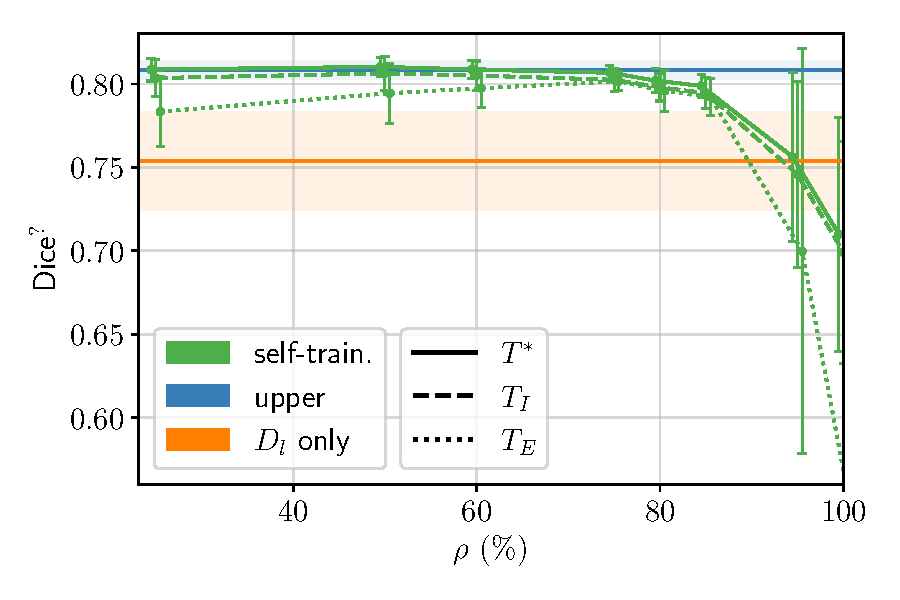
\includegraphics[width=\textwidth]{strain/manualtuning_monuseg_pred_entropy_none.pdf}
    \caption{\acrshort{monuseg}, entropy}
    \label{sfig:strain:manual:monu_entropy}
  \end{subfigure}
  \begin{subfigure}{0.48\textwidth}
    \centering
    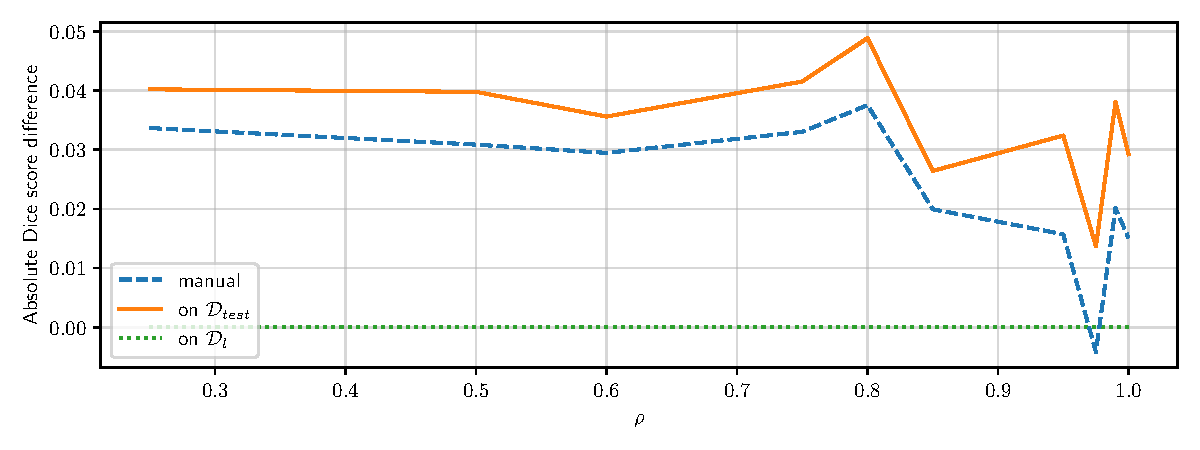
\includegraphics[width=\textwidth]{strain/manualtuning_monuseg_constant_1.0.pdf}
    \caption{\acrshort{monuseg}, constant ($C=1.0$)}
    \label{sfig:strain:manual:monu_constant}
  \end{subfigure} \\
  \begin{subfigure}{0.48\textwidth}
    \centering
    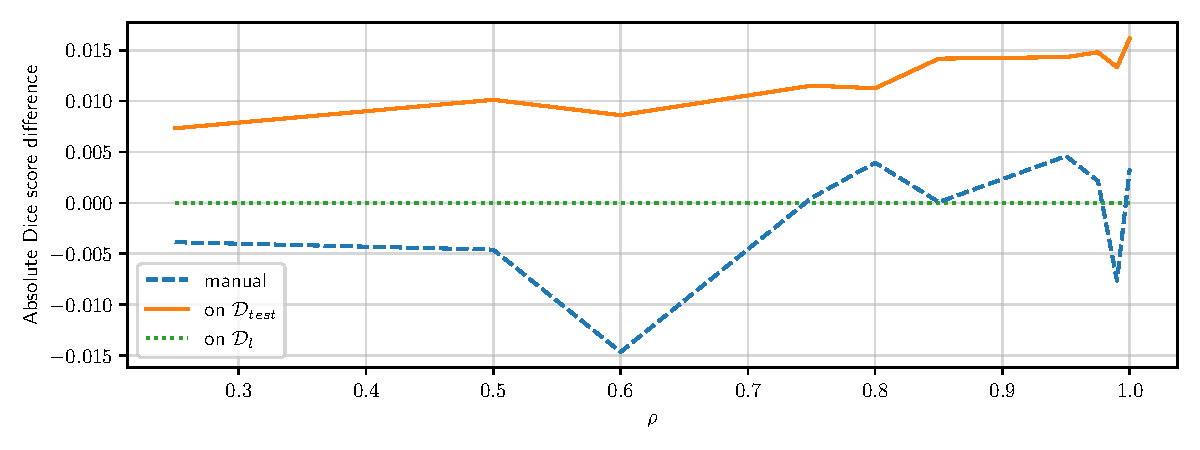
\includegraphics[width=\textwidth]{strain/manualtuning_glas_pred_entropy_none.pdf}
    \caption{\acrshort{glas}, entropy}
    \label{sfig:strain:manual:_glas_pred_entropy_none}
  \end{subfigure}
  \begin{subfigure}{0.48\textwidth}
    \centering
    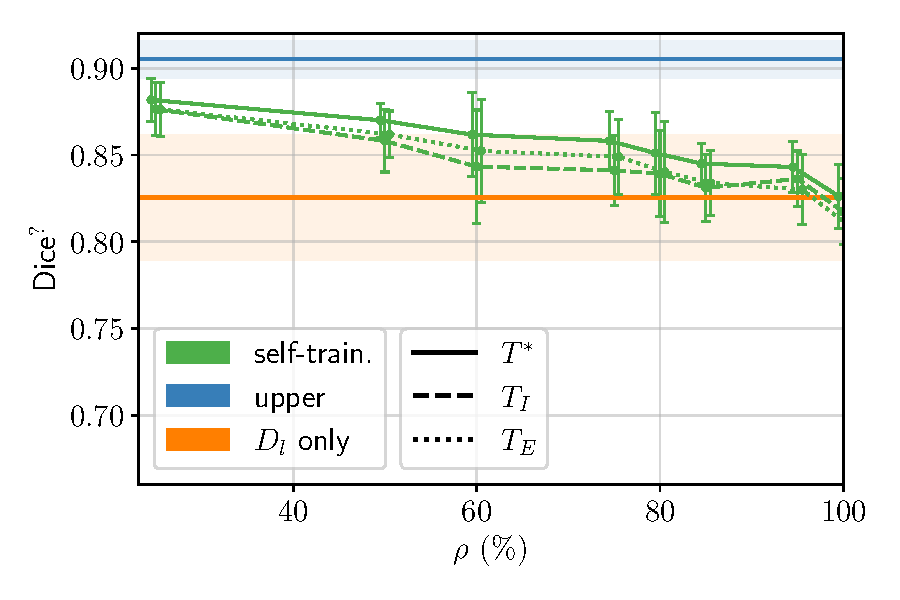
\includegraphics[width=\textwidth]{strain/manualtuning_glas_constant_0.5.pdf}
    \caption{\acrshort{glas}, constant ($C=0.5$)}
    \label{sfig:strain:manual:_glas_constant}
  \end{subfigure} \\
  \begin{subfigure}{0.48\textwidth}
    \centering
    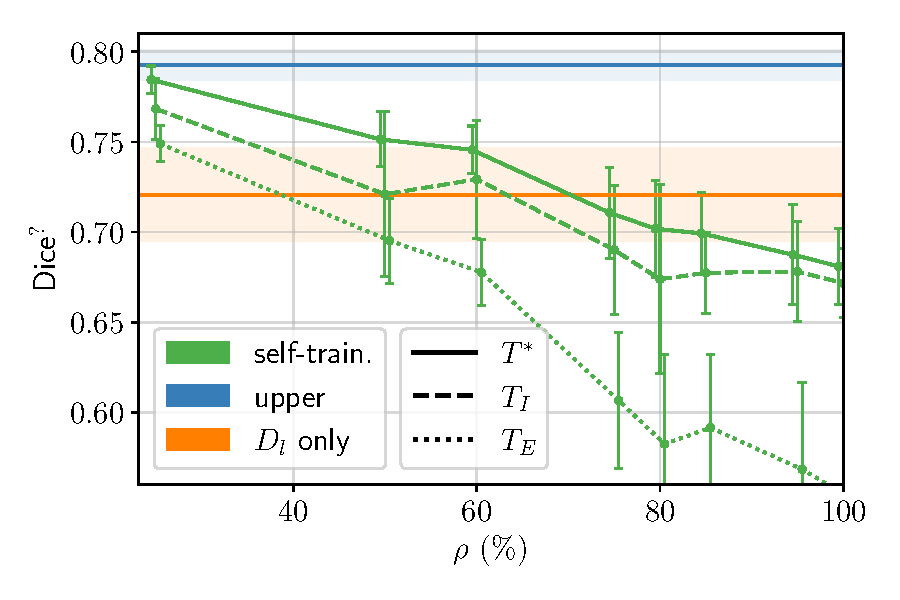
\includegraphics[width=\textwidth]{strain/manualtuning_segpc_pred_entropy_none.pdf}
    \caption{\acrshort{segpc}, entropy}
    \label{sfig:strain:manual:_segpc_pred_entropy_none}
  \end{subfigure}
  \begin{subfigure}{0.48\textwidth}
    \centering
    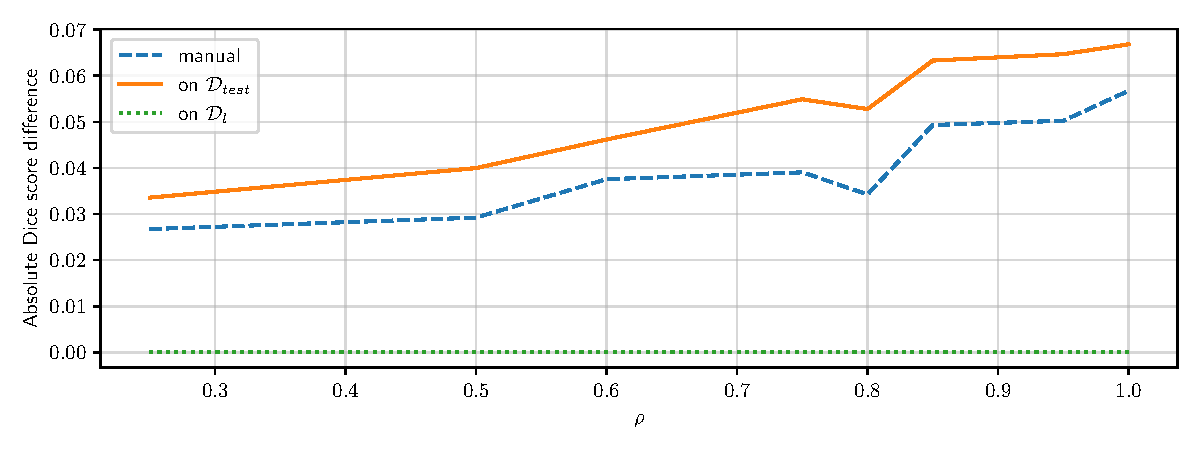
\includegraphics[width=\textwidth]{strain/manualtuning_segpc_constant_0.5.pdf}
    \caption{\acrshort{segpc}, constant ($C=0.5$)}
    \label{sfig:strain:manual:_segpc_constant}
  \end{subfigure}
  \caption{``Manual'' tuning performance. Reported values are the absolute Dice score differences between tuning $T$ on $\mathcal{D}_l$ (dotted green, reference) and approaches where $T$ is tuned on two test images (dashed blue), on the whole test set $\mathcal{D}_{test}$ (solid orange).}
  \label{fig:strain:manualtuning}

\end{figure}


\subsection{Experiment on Thyroid \acrshort{fnab}}
\label{ssec:strain:thyroid_exp}

As explained in Section \ref{ssec:strain:thyroidfnab}, the Thyroid \acrshort{fnab} dataset presents a great opportunity to test our dataset on a real case of sparse annotations. It is also interesting to note that this dataset is not only larger (almost 5k images total) than the three public datasets used in this study but also features both a validation set and a test set. Therefore, it allows for additional tuning of hyperparameters. In this experiment, we propose to evaluate the effect of early stopping and tuning the segmentation threshold on the validation set. We also select the best self-training hyperparameters combination on this validation set (\ie notably the weight strategy and its hyperparameters, the evaluated combinations can be found in the Supplementary \TODO{supp}). We compare the best self-training approach with two of our three baselines: $\mathcal{D}_l$ only and $\mathcal{D}_l \cup \mathcal{D}_s$. The upper baseline obviously cannot be evaluated because we do not have access to the complete ground truth. For both baselines, we also evaluate the effects of early stopping and threshold tuning with the validation set. The resulting performances are given in Table \ref{tab:strain:thyroidresults}.

\TODO{done with only one random seed???}
\TODO{validation and test sets are not very consistent -> in the (no, no) experiment, the baselines should not exhibit such a different variations between validation and test set as nothing is optimized on the validation set. There seems to be major discrepencies between both sets.}

We observe that the best self-training approach always outperforms the two baselines and remains quite stable whether or not we perform early stopping or threshold optimization on the validation set. 

\begin{table}
  \centering 
  \footnotesize
  \begin{tabular}{|cc|ccc|ccc|ccc|}
    \hline
    Early & Val. & \multicolumn{3}{c|}{Validation score} & \multicolumn{3}{c|}{Test score} & \multicolumn{3}{c|}{Best self-training approach} \\
    stopping & thresh. & $\mathcal{D}_l$ only & $\mathcal{D}_l \cup \mathcal{D}_s$ & Self-train. & $\mathcal{D}_l$ only & $\mathcal{D}_l \cup \mathcal{D}_s$ & Self-train. & H/S & Weights & Params \\
    \hline
    no & no & 62.29 & 59.90 & 80.01 & 75.17 & 80.65 & 85.12 & soft & merged & $w_{min}=0.1$ \\
    no & yes & 63.43 & 64.66 & 86.64 & 83.58 & 80.65 & 84.71 & soft & merged & $w_{min}=0.1$ \\  
    yes & no & 81.45 & 82.33 & 83.66 & 84.73 & 84.22 & 85.71 & hard & entropy & $w_{min}=0.75$ \\
    yes & yes & 87.05 & 87.66 & 89.10 & 84.73 & 84.38 & 85.24 & hard & merged & $w_{min}=0.5$ \\
    \hline
  \end{tabular}
  \caption{Experiment on the Thyroid \acrshort{fnab} dataset with/without early stopping and threshold optimization on the validation set (\textit{Val. thresh.}). \textit{H/S} stands for Hard/Soft labels.}
  \label{tab:strain:thyroidresults}
\end{table}



\section{Discussion and conclusion}

\parencite{haridas2015interactive, petit2018handling, petit2021iterative}